\documentclass[a4paper,11pt]{article}
\usepackage[utf8]{inputenc}
\usepackage{listings}
\usepackage{mathtools}   % need for subequations
\usepackage{graphicx}   % need for figures
\usepackage{verbatim}   % useful for program listings
\usepackage{color}      % use if color is used in text
\usepackage{hyperref}  
\usepackage{url}
\usepackage{float}
\usepackage{todonotes}
\usepackage{tikz}
\usepackage{enumitem}
\usepackage{hyperref}
\usepackage{pdfpages}
\usepackage{caption}
\usepackage{subcaption}
\usepackage{listings}
\usepackage{color}
\usepackage{amsfonts}
\usepackage{latexsym}
\usepackage[T1]{fontenc} % use for allowing < and > in cleartext
\usepackage{fixltx2e}    % use for textsubscript

\usepackage[margin=2.5cm]{geometry}
\usepackage[ampersand]{easylist}
\usepackage{tikz}
\usepackage{epstopdf}

\bibliographystyle{plain}

\begin{document}
\setlength{\parindent}{0cm}
\setlength{\unitlength}{1mm}
\date{December 17th 2014\\ IT University of Copenhagen}
\title{Roles In Movies\\SAD2 Fall 2014}

\author{Sarah de Voss\\
\texttt{satv@itu.dk}
\and Elvis Flesborg\\
\texttt{efle@itu.dk}
\and Mads Westi\\
\texttt{mwek@itu.dk}}
\clearpage\maketitle
\newpage
\thispagestyle{empty}
\setcounter{page}{1}
\tableofcontents
\newpage

\section{The method acting problem}
Acting is hard, the specific branch of method acting\footnote{Actors use this technique to create in themselves the thoughts and feelings of their role} appear even harder. Whenever an actor has finished playing a role, the process of creating a character starts all over. This is time consuming and inefficient, but what if the actor could use parts of his or hers current role? We want to construct an algorithm that gives actors clues to which roles to audition for next, by measuring the similarity between roles. We have dubbed this similarity search problem the "Method acting problem".


\section{Implementation}
We assume that there is a high correlation between the distinct roles in a movie and the rating the movie receives. Because the success of an actor is dependent on, whether he or she appears in high ranked movies, therefore movies with $rank \leq 7.0$ is purged from the data.

We will look at the naïve solution, then \emph{MinHashing}, and then \emph{Locality Sensitive Hashing}, this is part one of the report. After that we will implement \emph{b-bit} and \emph{odd sketch}, which is the extension to our report.


\subsection{Measuring similarity}
Since a role is represented as a set movies, we can measure the similarity between roles using the Jaccard similarity, where the similarity between two sets $S_1$ and $S_2$.

\begin{equation}
Sim(S_1, S_2) = \frac{|S_1 \cap S_2|}{|S_1 \cup S_2|}
\end{equation}
The Jaccard index falls in the range of 0-1. It is 1 if the sets are similar, and it is 0 if the sets are disjoint.


\subsection{Measuring Running Time}
For every new implementation, we will measure the actual running time. It will be measured on a normal laptop computer with 8GB RAM and and intel i5 quadcore. Though, if the running time is taking longer than out patience permits, we will just put in how long we waited, and note that we did not run it through.

We will also create some random dummy data to run. This way we will be able to graph the running times, and look at the tendency curves. In the dummy data, there are 10 times as many roles, as there are movies. This corresponds pretty well with the \emph{imdb-r.txt} file, which has 57,736 distinct movies, and 553,263 distinct roles (not counting the movies without any roles and roles with nonexisting movie-ids).

But even though there are 10 more roles per movies. Many of these roles are only in one movie, and only few roles are in many movies. If we calculate the average number of movies, that a role appears in, it is somewhere between 1.2 and 2.0, depending on what our cut-off rank is (see figure ~\ref{fig:sparsenesscutoff}. We have defined our minimum rank cutoff to movies with at least 7.0 in rank, which corresponds to an average of 1.7 movies per role. This has influence on the characteristic matrix, that we create when parsing.

This will be taken into account when creating our random dummy data.

\begin{figure}[!htbp]
    \begin{center}
        % GNUPLOT: LaTeX picture with Postscript
\begingroup
  \makeatletter
  \providecommand\color[2][]{%
    \GenericError{(gnuplot) \space\space\space\@spaces}{%
      Package color not loaded in conjunction with
      terminal option `colourtext'%
    }{See the gnuplot documentation for explanation.%
    }{Either use 'blacktext' in gnuplot or load the package
      color.sty in LaTeX.}%
    \renewcommand\color[2][]{}%
  }%
  \providecommand\includegraphics[2][]{%
    \GenericError{(gnuplot) \space\space\space\@spaces}{%
      Package graphicx or graphics not loaded%
    }{See the gnuplot documentation for explanation.%
    }{The gnuplot epslatex terminal needs graphicx.sty or graphics.sty.}%
    \renewcommand\includegraphics[2][]{}%
  }%
  \providecommand\rotatebox[2]{#2}%
  \@ifundefined{ifGPcolor}{%
    \newif\ifGPcolor
    \GPcolorfalse
  }{}%
  \@ifundefined{ifGPblacktext}{%
    \newif\ifGPblacktext
    \GPblacktexttrue
  }{}%
  % define a \g@addto@macro without @ in the name:
  \let\gplgaddtomacro\g@addto@macro
  % define empty templates for all commands taking text:
  \gdef\gplbacktext{}%
  \gdef\gplfronttext{}%
  \makeatother
  \ifGPblacktext
    % no textcolor at all
    \def\colorrgb#1{}%
    \def\colorgray#1{}%
  \else
    % gray or color?
    \ifGPcolor
      \def\colorrgb#1{\color[rgb]{#1}}%
      \def\colorgray#1{\color[gray]{#1}}%
      \expandafter\def\csname LTw\endcsname{\color{white}}%
      \expandafter\def\csname LTb\endcsname{\color{black}}%
      \expandafter\def\csname LTa\endcsname{\color{black}}%
      \expandafter\def\csname LT0\endcsname{\color[rgb]{1,0,0}}%
      \expandafter\def\csname LT1\endcsname{\color[rgb]{0,1,0}}%
      \expandafter\def\csname LT2\endcsname{\color[rgb]{0,0,1}}%
      \expandafter\def\csname LT3\endcsname{\color[rgb]{1,0,1}}%
      \expandafter\def\csname LT4\endcsname{\color[rgb]{0,1,1}}%
      \expandafter\def\csname LT5\endcsname{\color[rgb]{1,1,0}}%
      \expandafter\def\csname LT6\endcsname{\color[rgb]{0,0,0}}%
      \expandafter\def\csname LT7\endcsname{\color[rgb]{1,0.3,0}}%
      \expandafter\def\csname LT8\endcsname{\color[rgb]{0.5,0.5,0.5}}%
    \else
      % gray
      \def\colorrgb#1{\color{black}}%
      \def\colorgray#1{\color[gray]{#1}}%
      \expandafter\def\csname LTw\endcsname{\color{white}}%
      \expandafter\def\csname LTb\endcsname{\color{black}}%
      \expandafter\def\csname LTa\endcsname{\color{black}}%
      \expandafter\def\csname LT0\endcsname{\color{black}}%
      \expandafter\def\csname LT1\endcsname{\color{black}}%
      \expandafter\def\csname LT2\endcsname{\color{black}}%
      \expandafter\def\csname LT3\endcsname{\color{black}}%
      \expandafter\def\csname LT4\endcsname{\color{black}}%
      \expandafter\def\csname LT5\endcsname{\color{black}}%
      \expandafter\def\csname LT6\endcsname{\color{black}}%
      \expandafter\def\csname LT7\endcsname{\color{black}}%
      \expandafter\def\csname LT8\endcsname{\color{black}}%
    \fi
  \fi
  \setlength{\unitlength}{0.0500bp}%
  \begin{picture}(7200.00,5040.00)%
    \gplgaddtomacro\gplbacktext{%
      \csname LTb\endcsname%
      \put(946,704){\makebox(0,0)[r]{\strut{} 1.2}}%
      \put(946,1156){\makebox(0,0)[r]{\strut{} 1.3}}%
      \put(946,1609){\makebox(0,0)[r]{\strut{} 1.4}}%
      \put(946,2061){\makebox(0,0)[r]{\strut{} 1.5}}%
      \put(946,2513){\makebox(0,0)[r]{\strut{} 1.6}}%
      \put(946,2966){\makebox(0,0)[r]{\strut{} 1.7}}%
      \put(946,3418){\makebox(0,0)[r]{\strut{} 1.8}}%
      \put(946,3870){\makebox(0,0)[r]{\strut{} 1.9}}%
      \put(946,4323){\makebox(0,0)[r]{\strut{} 2}}%
      \put(946,4775){\makebox(0,0)[r]{\strut{} 2.1}}%
      \put(1078,484){\makebox(0,0){\strut{} 0}}%
      \put(2223,484){\makebox(0,0){\strut{} 2}}%
      \put(3368,484){\makebox(0,0){\strut{} 4}}%
      \put(4513,484){\makebox(0,0){\strut{} 6}}%
      \put(5658,484){\makebox(0,0){\strut{} 8}}%
      \put(6803,484){\makebox(0,0){\strut{} 10}}%
      \put(176,2739){\rotatebox{-270}{\makebox(0,0){\strut{}Average movies per role}}}%
      \put(3940,154){\makebox(0,0){\strut{}minimum rank}}%
    }%
    \gplgaddtomacro\gplfronttext{%
    }%
    \gplbacktext
    \put(0,0){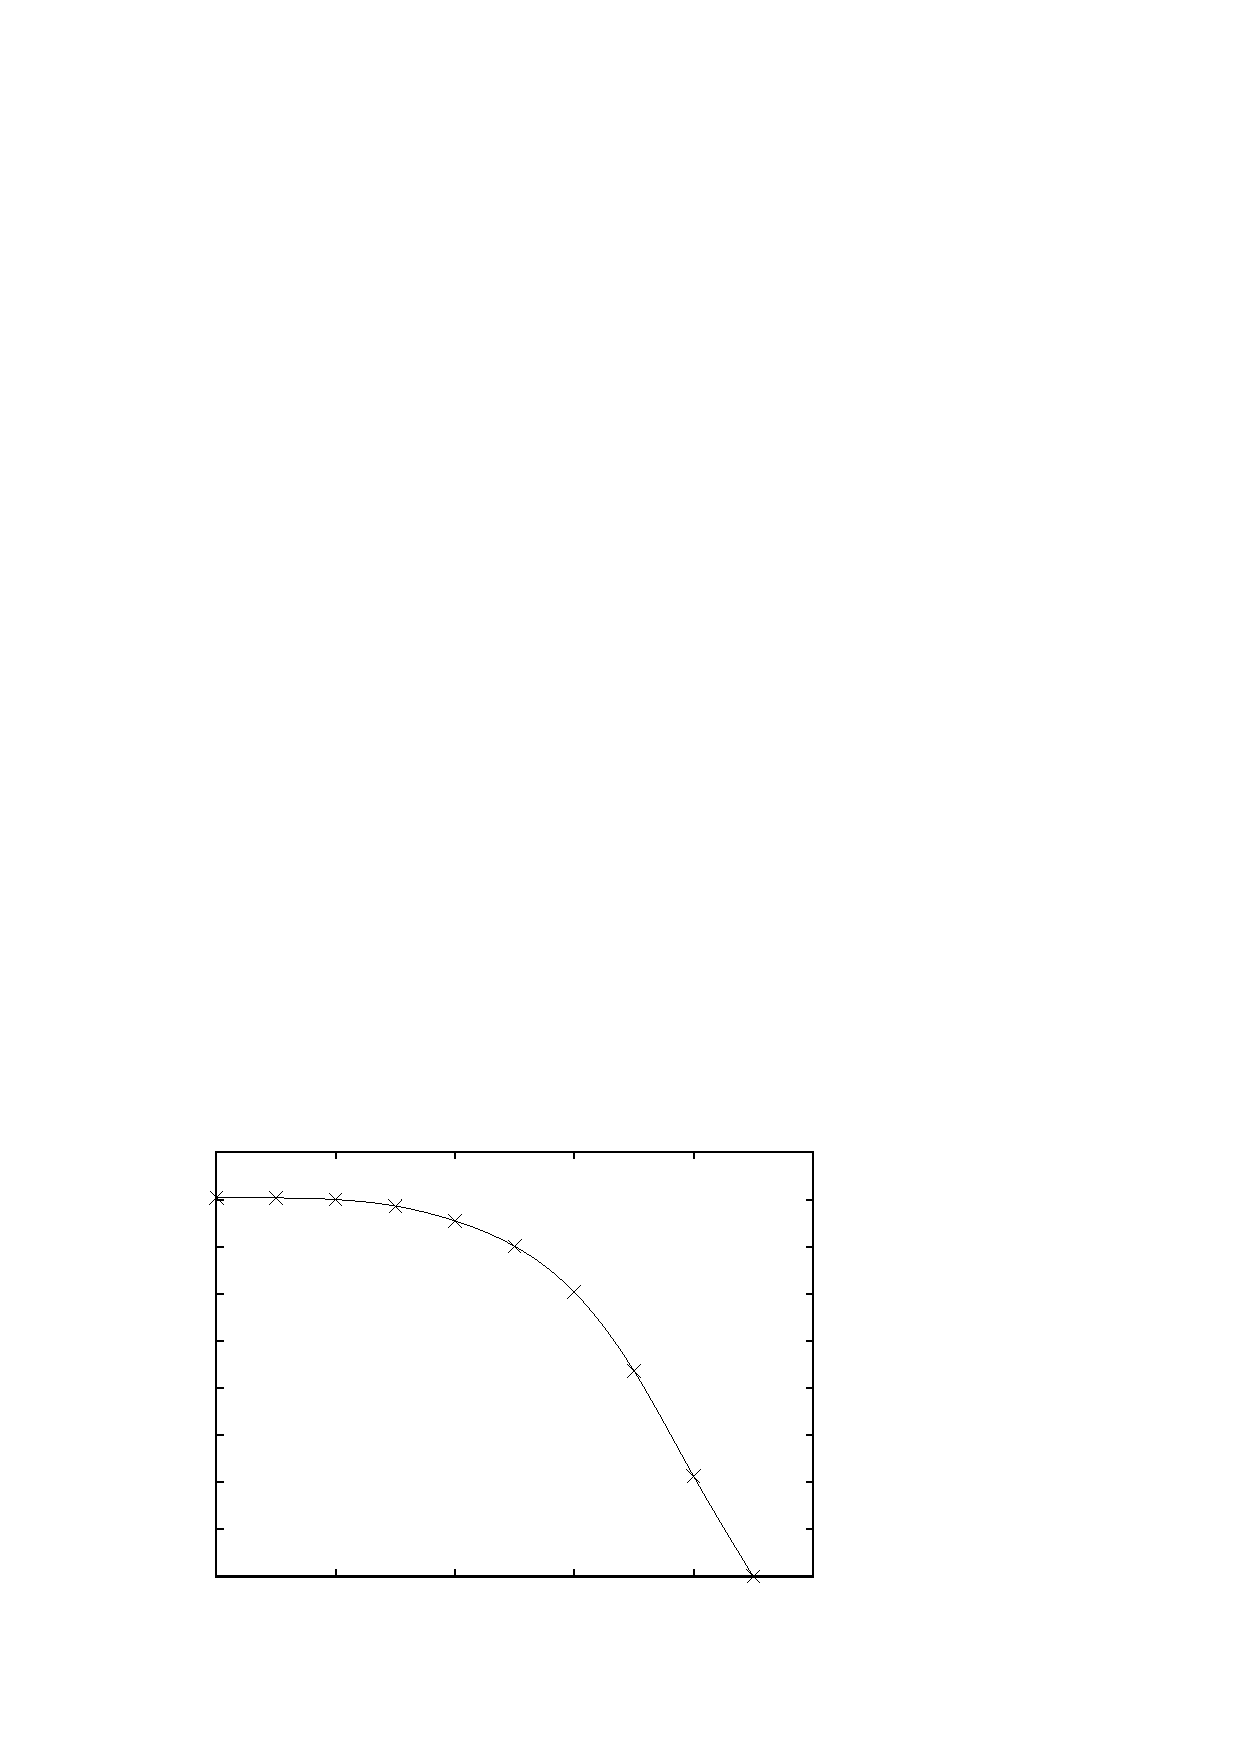
\includegraphics{plots/ones_per_role}}%
    \gplfronttext
  \end{picture}%
\endgroup

        \caption{Sparseness with cutoff}
        \label{fig:sparsenesscutoff}
    \end{center}
\end{figure}

\subsection{Naïve Implementation}

\subsubsection{Data representation}
A role is represented as a list of movies\footnote{Corresponding to the ids of the movies, which is integers} the specific role appear in.

\begin{equation}
r_1 = \{m_1, m_2, m_3, \ldots , m_i\}
\end{equation}

The data is stored in a characteristic matrix, where the rows are movies and the columns are roles.

\begin{figure}[!htbp]
\begin{eqnarray*}
 & n \ \text{roles} \\
 m \ \text{movies} = & 
\begin{cases}
    \overbrace{
    \begin{bmatrix}
        1 & 0 & 1 & 0 & 0 & 0 & 1\\
        1 & 0 & 0 & 1 & 0 & 0 & 1\\
        0 & 1 & 0 & 1 & 0 & 1 & 0\\
        0 & 1 & 0 & 1 & 0 & 0 & 0\\
        0 & 1 & 0 & 1 & 0 & 0 & 1\\
        1 & 0 & 1 & 0 & 0 & 0 & 1\\
        1 & 0 & 1 & 0 & 1 & 0 & 0
    \end{bmatrix} 
    }
\end{cases}
\end{eqnarray*}
\caption{The characteristic matrix}
\label{fig:char_matrix}
\end{figure}

To save space in memory, we do not save the matrix as it is seen in ~\ref{fig:char_matrix}. We save a list of the pairs that have a 1 in common, as suggested in \cite{book:mmds} p. 81. Worst case, the space consumption would be $O(n \times m)$ \ \footnote{If every role was in every movie}, but since we have a very sparse characteristic matrix, we save a lot of space doing this. \\

Because we have to permute every possible pair of roles, the running time is $O(n^2 \cdot m)$, where $n$ is the number of distinct roles, and $m$ is the number of movies. In a scenario where $m$ is almost equal to $n$, the runtime will be $O(n^3)$. \\

This will surely not fit in memory with the whole dataset, so more sofisticated algorithms are needed. \\

\subsubsection{Actual Running Time}
The actual running time with the naïve implementation takes too long for our normal laptop computer to outrun our patience. We ran the implementation on random dummy datasets, which can be seen in figure ~\ref{fig:naive_at}.

\begin{figure}[!htbp]
    \begin{center}
        % GNUPLOT: LaTeX picture with Postscript
\begingroup
  \makeatletter
  \providecommand\color[2][]{%
    \GenericError{(gnuplot) \space\space\space\@spaces}{%
      Package color not loaded in conjunction with
      terminal option `colourtext'%
    }{See the gnuplot documentation for explanation.%
    }{Either use 'blacktext' in gnuplot or load the package
      color.sty in LaTeX.}%
    \renewcommand\color[2][]{}%
  }%
  \providecommand\includegraphics[2][]{%
    \GenericError{(gnuplot) \space\space\space\@spaces}{%
      Package graphicx or graphics not loaded%
    }{See the gnuplot documentation for explanation.%
    }{The gnuplot epslatex terminal needs graphicx.sty or graphics.sty.}%
    \renewcommand\includegraphics[2][]{}%
  }%
  \providecommand\rotatebox[2]{#2}%
  \@ifundefined{ifGPcolor}{%
    \newif\ifGPcolor
    \GPcolorfalse
  }{}%
  \@ifundefined{ifGPblacktext}{%
    \newif\ifGPblacktext
    \GPblacktexttrue
  }{}%
  % define a \g@addto@macro without @ in the name:
  \let\gplgaddtomacro\g@addto@macro
  % define empty templates for all commands taking text:
  \gdef\gplbacktext{}%
  \gdef\gplfronttext{}%
  \makeatother
  \ifGPblacktext
    % no textcolor at all
    \def\colorrgb#1{}%
    \def\colorgray#1{}%
  \else
    % gray or color?
    \ifGPcolor
      \def\colorrgb#1{\color[rgb]{#1}}%
      \def\colorgray#1{\color[gray]{#1}}%
      \expandafter\def\csname LTw\endcsname{\color{white}}%
      \expandafter\def\csname LTb\endcsname{\color{black}}%
      \expandafter\def\csname LTa\endcsname{\color{black}}%
      \expandafter\def\csname LT0\endcsname{\color[rgb]{1,0,0}}%
      \expandafter\def\csname LT1\endcsname{\color[rgb]{0,1,0}}%
      \expandafter\def\csname LT2\endcsname{\color[rgb]{0,0,1}}%
      \expandafter\def\csname LT3\endcsname{\color[rgb]{1,0,1}}%
      \expandafter\def\csname LT4\endcsname{\color[rgb]{0,1,1}}%
      \expandafter\def\csname LT5\endcsname{\color[rgb]{1,1,0}}%
      \expandafter\def\csname LT6\endcsname{\color[rgb]{0,0,0}}%
      \expandafter\def\csname LT7\endcsname{\color[rgb]{1,0.3,0}}%
      \expandafter\def\csname LT8\endcsname{\color[rgb]{0.5,0.5,0.5}}%
    \else
      % gray
      \def\colorrgb#1{\color{black}}%
      \def\colorgray#1{\color[gray]{#1}}%
      \expandafter\def\csname LTw\endcsname{\color{white}}%
      \expandafter\def\csname LTb\endcsname{\color{black}}%
      \expandafter\def\csname LTa\endcsname{\color{black}}%
      \expandafter\def\csname LT0\endcsname{\color{black}}%
      \expandafter\def\csname LT1\endcsname{\color{black}}%
      \expandafter\def\csname LT2\endcsname{\color{black}}%
      \expandafter\def\csname LT3\endcsname{\color{black}}%
      \expandafter\def\csname LT4\endcsname{\color{black}}%
      \expandafter\def\csname LT5\endcsname{\color{black}}%
      \expandafter\def\csname LT6\endcsname{\color{black}}%
      \expandafter\def\csname LT7\endcsname{\color{black}}%
      \expandafter\def\csname LT8\endcsname{\color{black}}%
    \fi
  \fi
  \setlength{\unitlength}{0.0500bp}%
  \begin{picture}(7200.00,5040.00)%
    \gplgaddtomacro\gplbacktext{%
      \csname LTb\endcsname%
      \put(1078,704){\makebox(0,0)[r]{\strut{} 0}}%
      \put(1078,1383){\makebox(0,0)[r]{\strut{} 200}}%
      \put(1078,2061){\makebox(0,0)[r]{\strut{} 400}}%
      \put(1078,2740){\makebox(0,0)[r]{\strut{} 600}}%
      \put(1078,3418){\makebox(0,0)[r]{\strut{} 800}}%
      \put(1078,4097){\makebox(0,0)[r]{\strut{} 1000}}%
      \put(1078,4775){\makebox(0,0)[r]{\strut{} 1200}}%
      \put(1210,484){\makebox(0,0){\strut{} 0}}%
      \put(2329,484){\makebox(0,0){\strut{} 1}}%
      \put(3447,484){\makebox(0,0){\strut{} 2}}%
      \put(4566,484){\makebox(0,0){\strut{} 3}}%
      \put(5684,484){\makebox(0,0){\strut{} 4}}%
      \put(6803,484){\makebox(0,0){\strut{} 5}}%
      \put(176,2739){\rotatebox{-270}{\makebox(0,0){\strut{}Time (s)}}}%
      \put(4006,154){\makebox(0,0){\strut{}Input data size (x100 movies | x1000 actors)}}%
    }%
    \gplgaddtomacro\gplfronttext{%
    }%
    \gplbacktext
    \put(0,0){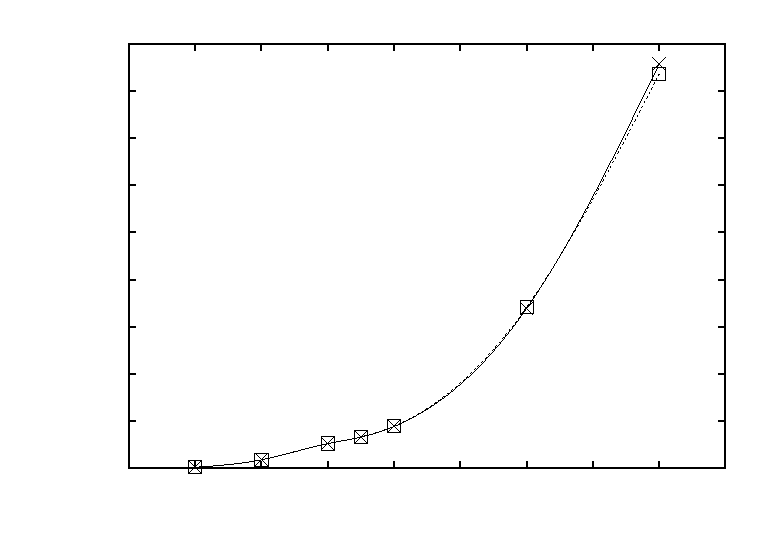
\includegraphics{plots/naive_at}}%
    \gplfronttext
  \end{picture}%
\endgroup

        \caption{Naïve Implementation Actual Times}
        \label{fig:naive_at}
    \end{center}
\end{figure}


\section{MinHashing}
Since the permutation of such a large matrix is infeasible, we create a number of hash functions, $h_1, ..., h_k$, which should be less than the number of rows in the characteristic matrix. To compare sets of documents, the normal procedure is to convert them into shingles. But since the "documents" we are working on, are actual sets of index numbers, there is no need for us to use shingles. \\

Remarkably, the probability that the minhash function produces the same value for two sets is the same as the Jaccard similarity of the two sets (p. 82 in \cite{book:mmds}). Let \\

    $x = $ the rows in which the two sets both have a 1. \\
    $y = $ the rows in which one of the sets have a 1. \\
    $z = $ the rows in which none of the sets have a 1. \\

Then the probability of having found a row in $x$, for a random permutation, is

\begin{equation*}
    \frac{x}{x+y}
\end{equation*}

which is equals to the Jaccard similarity of the two sets.

\begin{equation*}
    \frac{S_1 \cap S_2}{S_1 \cup S_2} = \frac{x}{x+y}
\end{equation*}
    
We simulate $k$ random permutations by creating $k$ number of random hash functions \footnote{We are using universal hashing ($(ax + b) \bmod p$) as our hashing functions, where there will be some collisions in the hashes. Some row indexes will be hashed to the same, but as long as $k$ is large it is not important (p. 83-84 in \cite{book:mmds}).}. All row indices are then hashed with all these hash functions, to simulate a permutation. When this is done, we have created the signature matrix, which is a $k\times n$ matrix, that contains the minimum value of $h(x)$, where $x$ is an element in $S$. See figure ~\ref{fig:signature_matrix}\\

\begin{figure}[!htpb]
    \begin{eqnarray*}
     & n \ \text{signatures} \\
     k \ \text{permutations} = & 
        \begin{cases}
        \overbrace{
        \begin{bmatrix}
            1 & 1 & 4 & 3 & 3 & 6 & 4\\
            3 & 3 & 1 & 5 & 3 & 2 & 1\\
            4 & 3 & 2 & 3 & 3 & 4 & 5\\
            0 & 1 & 4 & 2 & 2 & 6 & 1\\
        \end{bmatrix} 
        } 
        \end{cases}
    \end{eqnarray*}
    \caption{Signature matrix}
    \label{fig:signature_matrix}
\end{figure}

We still have to permute all pairs of roles, but the number of comparisons is reduced to $k$, the new running time is therefore $O(n^2 \cdot k)$ compared to $O(n^2 \cdot m)$ of the naïve solution, see figure ~\ref{fig:char_matrix} versus ~\ref{fig:signature_matrix}.

\subsection{Actual Running Times}
In figure ~\ref{fig:minhashing_at} the actual running times can be seen.


\begin{figure}[!htpb]
    \begin{center}
        % GNUPLOT: LaTeX picture with Postscript
\begingroup
  \makeatletter
  \providecommand\color[2][]{%
    \GenericError{(gnuplot) \space\space\space\@spaces}{%
      Package color not loaded in conjunction with
      terminal option `colourtext'%
    }{See the gnuplot documentation for explanation.%
    }{Either use 'blacktext' in gnuplot or load the package
      color.sty in LaTeX.}%
    \renewcommand\color[2][]{}%
  }%
  \providecommand\includegraphics[2][]{%
    \GenericError{(gnuplot) \space\space\space\@spaces}{%
      Package graphicx or graphics not loaded%
    }{See the gnuplot documentation for explanation.%
    }{The gnuplot epslatex terminal needs graphicx.sty or graphics.sty.}%
    \renewcommand\includegraphics[2][]{}%
  }%
  \providecommand\rotatebox[2]{#2}%
  \@ifundefined{ifGPcolor}{%
    \newif\ifGPcolor
    \GPcolorfalse
  }{}%
  \@ifundefined{ifGPblacktext}{%
    \newif\ifGPblacktext
    \GPblacktexttrue
  }{}%
  % define a \g@addto@macro without @ in the name:
  \let\gplgaddtomacro\g@addto@macro
  % define empty templates for all commands taking text:
  \gdef\gplbacktext{}%
  \gdef\gplfronttext{}%
  \makeatother
  \ifGPblacktext
    % no textcolor at all
    \def\colorrgb#1{}%
    \def\colorgray#1{}%
  \else
    % gray or color?
    \ifGPcolor
      \def\colorrgb#1{\color[rgb]{#1}}%
      \def\colorgray#1{\color[gray]{#1}}%
      \expandafter\def\csname LTw\endcsname{\color{white}}%
      \expandafter\def\csname LTb\endcsname{\color{black}}%
      \expandafter\def\csname LTa\endcsname{\color{black}}%
      \expandafter\def\csname LT0\endcsname{\color[rgb]{1,0,0}}%
      \expandafter\def\csname LT1\endcsname{\color[rgb]{0,1,0}}%
      \expandafter\def\csname LT2\endcsname{\color[rgb]{0,0,1}}%
      \expandafter\def\csname LT3\endcsname{\color[rgb]{1,0,1}}%
      \expandafter\def\csname LT4\endcsname{\color[rgb]{0,1,1}}%
      \expandafter\def\csname LT5\endcsname{\color[rgb]{1,1,0}}%
      \expandafter\def\csname LT6\endcsname{\color[rgb]{0,0,0}}%
      \expandafter\def\csname LT7\endcsname{\color[rgb]{1,0.3,0}}%
      \expandafter\def\csname LT8\endcsname{\color[rgb]{0.5,0.5,0.5}}%
    \else
      % gray
      \def\colorrgb#1{\color{black}}%
      \def\colorgray#1{\color[gray]{#1}}%
      \expandafter\def\csname LTw\endcsname{\color{white}}%
      \expandafter\def\csname LTb\endcsname{\color{black}}%
      \expandafter\def\csname LTa\endcsname{\color{black}}%
      \expandafter\def\csname LT0\endcsname{\color{black}}%
      \expandafter\def\csname LT1\endcsname{\color{black}}%
      \expandafter\def\csname LT2\endcsname{\color{black}}%
      \expandafter\def\csname LT3\endcsname{\color{black}}%
      \expandafter\def\csname LT4\endcsname{\color{black}}%
      \expandafter\def\csname LT5\endcsname{\color{black}}%
      \expandafter\def\csname LT6\endcsname{\color{black}}%
      \expandafter\def\csname LT7\endcsname{\color{black}}%
      \expandafter\def\csname LT8\endcsname{\color{black}}%
    \fi
  \fi
  \setlength{\unitlength}{0.0500bp}%
  \begin{picture}(7200.00,5040.00)%
    \gplgaddtomacro\gplbacktext{%
      \csname LTb\endcsname%
      \put(946,704){\makebox(0,0)[r]{\strut{} 0}}%
      \put(946,1286){\makebox(0,0)[r]{\strut{} 50}}%
      \put(946,1867){\makebox(0,0)[r]{\strut{} 100}}%
      \put(946,2449){\makebox(0,0)[r]{\strut{} 150}}%
      \put(946,3030){\makebox(0,0)[r]{\strut{} 200}}%
      \put(946,3612){\makebox(0,0)[r]{\strut{} 250}}%
      \put(946,4193){\makebox(0,0)[r]{\strut{} 300}}%
      \put(946,4775){\makebox(0,0)[r]{\strut{} 350}}%
      \put(1078,484){\makebox(0,0){\strut{} 0}}%
      \put(1714,484){\makebox(0,0){\strut{} 1}}%
      \put(2350,484){\makebox(0,0){\strut{} 2}}%
      \put(2986,484){\makebox(0,0){\strut{} 3}}%
      \put(3622,484){\makebox(0,0){\strut{} 4}}%
      \put(4259,484){\makebox(0,0){\strut{} 5}}%
      \put(4895,484){\makebox(0,0){\strut{} 6}}%
      \put(5531,484){\makebox(0,0){\strut{} 7}}%
      \put(6167,484){\makebox(0,0){\strut{} 8}}%
      \put(6803,484){\makebox(0,0){\strut{} 9}}%
      \put(176,2739){\rotatebox{-270}{\makebox(0,0){\strut{}Time (s)}}}%
      \put(3940,154){\makebox(0,0){\strut{}Input data size (x100 movies | x1000 roles)}}%
    }%
    \gplgaddtomacro\gplfronttext{%
      \csname LTb\endcsname%
      \put(2704,4083){\makebox(0,0)[r]{\strut{}k=5}}%
      \csname LTb\endcsname%
      \put(2704,3863){\makebox(0,0)[r]{\strut{}k=10}}%
      \csname LTb\endcsname%
      \put(2704,3643){\makebox(0,0)[r]{\strut{}k=20}}%
      \csname LTb\endcsname%
      \put(2704,3423){\makebox(0,0)[r]{\strut{}k=40}}%
    }%
    \gplbacktext
    \put(0,0){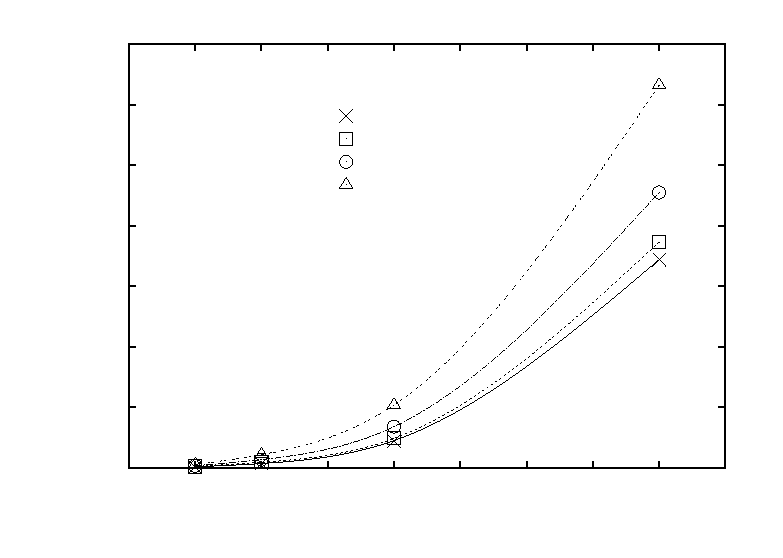
\includegraphics{plots/minhashing_at}}%
    \gplfronttext
  \end{picture}%
\endgroup

        \caption{MinHashing Actual Times}
        \label{fig:minhashing_at}
    \end{center}
\end{figure}


\section{Locality Sensitive Hashing (LSH)}
Locality sensitive hashing is a way of coping with an even larger amount of data than MinHashing can. So if the number of pairs is too large, LSH is an option to use. We take the signatures produced by min hashing and chop them up into shorter vectors by dividing the total number of rows into $b$ bands of $r$ rows. We then hash the vectors into a large number of buckets. If 2 vectors hash to the same bucket there is a good chance that they are similar. These vectors become candidate pairs, and we only compare candidate pairs for similarity. This leaves us with a significant fraction of the original set of pairs to check. \\

When choosing the number of bands, it is important to keeping in mind that we want few false negatives/positives. We can compute the probability of a particular pair becoming a candidate pair by using the S-curve equation. $s$ is the probability that 2 signatures become a candidate pair.

\begin{equation}
    \text {S-curve equation} = 1 - (1 - s^r)^b 
\end{equation}\\

The steepest point on the curve, is the spot where the ratio between false positives and false negatives is $1:1$. This point can be estimated with equation \ref{eq:s-estimate}.

\begin{equation}
    s = (1/b)^{1/r}
    \label{eq:s-estimate}
\end{equation}


\begin{figure}
    \begin{center}
        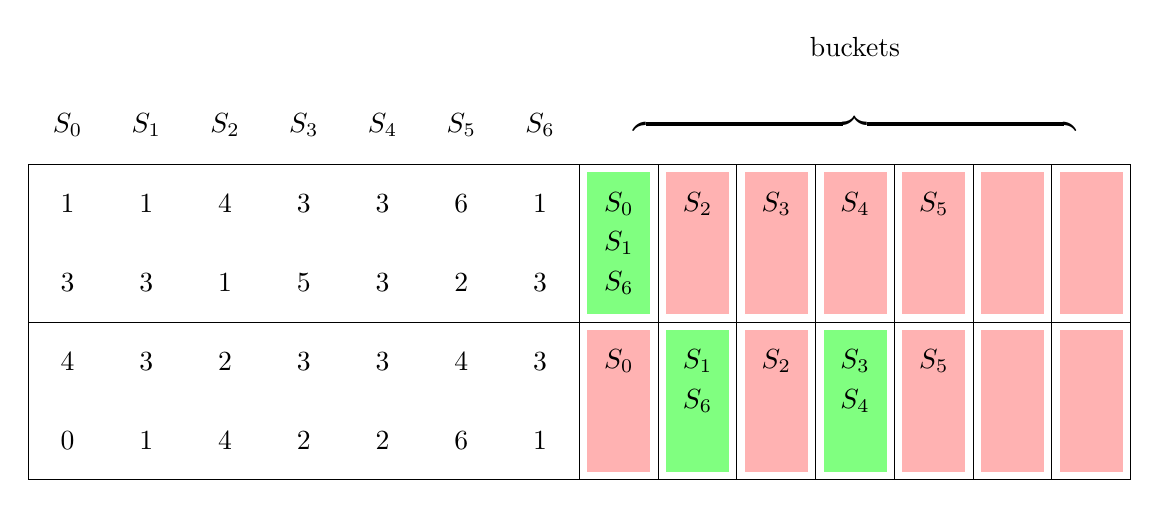
\begin{tikzpicture}
            \draw rectangle (14,4);
            \draw rectangle (7,2);
            \draw (0,2) rectangle (7,2);
            \draw (7,0) rectangle (8,4);

            \foreach \x in {0,...,6} \draw (\x+7, 0) rectangle (\x+7+1, 2);
            \foreach \x in {0,...,6} \draw (\x+7, 2) rectangle (\x+7+1, 4);
            \foreach \x in {0,...,6} \draw (\x+.5, 4.5) node {$S_\x$};

            \draw (10.5, 4.5) node {$\overbrace{\qquad\qquad\qquad\qquad\qquad\qquad\qquad\qquad}$};
            \draw (10.5,5.5) node {buckets};

            \draw (0.5,3.5) node {1};
            \draw (0.5,2.5) node {3};
            \draw (0.5,1.5) node {4};
            \draw (0.5,0.5) node {0};

            \draw (1.5,3.5) node {1};
            \draw (1.5,2.5) node {3};
            \draw (1.5,1.5) node {3};
            \draw (1.5,0.5) node {1};

            \draw (2.5,3.5) node {4};
            \draw (2.5,2.5) node {1};
            \draw (2.5,1.5) node {2};
            \draw (2.5,0.5) node {4};

            \draw (3.5,3.5) node {3};
            \draw (3.5,2.5) node {5};
            \draw (3.5,1.5) node {3};
            \draw (3.5,0.5) node {2};

            \draw (4.5,3.5) node {3};
            \draw (4.5,2.5) node {3};
            \draw (4.5,1.5) node {3};
            \draw (4.5,0.5) node {2};

            \draw (5.5,3.5) node {6};
            \draw (5.5,2.5) node {2};
            \draw (5.5,1.5) node {4};
            \draw (5.5,0.5) node {6};

            \draw (6.5,3.5) node {1};
            \draw (6.5,2.5) node {3};
            \draw (6.5,1.5) node {3};
            \draw (6.5,0.5) node {1};

            \foreach \x in {0,...,6} \path[fill=red!30] (7.1+\x,0.1) rectangle (7.9+\x,1.9);
            \foreach \x in {0,...,6} \path[fill=red!30] (7.1+\x,2.1) rectangle (7.9+\x,3.9);

            \path[fill=green!50] (7.1,2.1) rectangle (7.9,3.9);
            \path[fill=green!50] (8.1,0.1) rectangle (8.9,1.9);
            \path[fill=green!50] (10.1,0.1) rectangle (10.9,1.9);

            \draw (7.5,3.5) node {$S_0$};
            \draw (7.5,3.0) node {$S_1$};
            \draw (7.5,2.5) node {$S_6$};
            \draw (8.5,3.5) node {$S_2$};
            \draw (9.5,3.5) node {$S_3$};
            \draw (10.5,3.5) node {$S_4$};
            \draw (11.5,3.5) node {$S_5$};

            \draw (7.5,1.5) node {$S_0$};
            \draw (8.5,1.5) node {$S_1$};
            \draw (8.5,1.0) node {$S_6$};
            \draw (9.5,1.5) node {$S_2$};
            \draw (10.5,1.5) node {$S_3$};
            \draw (10.5,1.0) node {$S_4$};
            \draw (11.5,1.5) node {$S_5$};

        \end{tikzpicture}
    \caption{LSH buckets}
    \label{fig:lsh_buckets}
    \end{center}
\end{figure}



How much accuracy do we sacrifice in percent?\\

Run time analysis/space complexity
While the use of minhashing reduces the running time of the similarity calculations. It is still not fesible to use the algorithm on the IMDB data set. The general idea of LSH is that before making comparisions, the signtures are hashed in such a way that similar signatures are hashed to the same buckets, resulting in candidate pairs for comparision.\\

If you were an algorithm which algorithm would you be?

\section{B-bit}
B-bit minwise hashing is a way to estimate set similarity in a more storage efficient way than with min hashing.
\section{Odd sketch}

\section{Conclusion}
\newpage
\bibliography{bibliography}
\end{document}





